\documentclass{tufte-book}

%BOOK METADATA
\title{HBase Code Crack}
\author[Dong Dai]{Dong Dai}
\publisher{Apache Licence}

\usepackage{lipsum}
\usepackage{booktabs}
\usepackage{graphicx}
\setkeys{Gin}{width=\linewidth,totalheight=\textheight,keepaspectratio}
\graphicspath{{graphics/}}

\usepackage{fancyvrb}
\fvset{fontsize=\normalsize}

\newcommand{\hangp}[1]{\makebox[0pt][r]{(}#1\makebox[0pt][l]{)}}
\newcommand{\hangstar}{\makebox[0pt][l]{*}}

\usepackage{xspace}
\newcommand{\vdqi}{\textit{VDQI}\xspace}
\newcommand{\ei}{\textit{EI}\xspace}
\newcommand{\ve}{\textit{VE}\xspace}
\newcommand{\be}{\textit{BE}\xspace}
\newcommand{\VDQI}{\textit{The Visual Display of Quantitative Information}\xspace}
\newcommand{\EI}{\textit{Envisioning Information}\xspace}
\newcommand{\VE}{\textit{Visual Explanations}\xspace}
\newcommand{\BE}{\textit{Beautiful Evidence}\xspace}
\newcommand{\TL}{Tufte-\LaTeX\xspace}

% Prints the month name (e.g., January) and the year (e.g., 2008)
\newcommand{\monthyear}{%
  \ifcase\month\or January\or February\or March\or April\or May\or June\or
  July\or August\or September\or October\or November\or
  December\fi\space\number\year
}


% Prints an epigraph and speaker in sans serif, all-caps type.
\newcommand{\openepigraph}[2]{%
  %\sffamily\fontsize{14}{16}\selectfont
  \begin{fullwidth}
  \sffamily\large
  \begin{doublespace}
  \noindent\allcaps{#1}\\% epigraph
  \noindent\allcaps{#2}% author
  \end{doublespace}
  \end{fullwidth}
}

% Inserts a blank page
\newcommand{\blankpage}{\newpage\hbox{}\thispagestyle{empty}\newpage}

\usepackage{units}

\newcommand{\measure}[3]{#1/#2$\times$\unit[#3]{pc}}

% Macros for typesetting the documentation
\newcommand{\hlred}[1]{\textcolor{Maroon}{#1}}% prints in red
\newcommand{\hangleft}[1]{\makebox[0pt][r]{#1}}
\newcommand{\hairsp}{\hspace{1pt}}% hair space
\newcommand{\hquad}{\hskip0.5em\relax}% half quad space
\newcommand{\TODO}{\textcolor{red}{\bf TODO!}\xspace}
\newcommand{\ie}{\textit{i.\hairsp{}e.}\xspace}
\newcommand{\eg}{\textit{e.\hairsp{}g.}\xspace}
\newcommand{\na}{\quad--}% used in tables for N/A cells
\providecommand{\XeLaTeX}{X\lower.5ex\hbox{\kern-0.15em\reflectbox{E}}\kern-0.1em\LaTeX}
\newcommand{\tXeLaTeX}{\XeLaTeX\index{XeLaTeX@\protect\XeLaTeX}}
% \index{\texttt{\textbackslash xyz}@\hangleft{\texttt{\textbackslash}}\texttt{xyz}}
\newcommand{\tuftebs}{\symbol{'134}}% a backslash in tt type in OT1/T1
\newcommand{\doccmdnoindex}[2][]{\texttt{\tuftebs#2}}% command name -- adds backslash automatically (and doesn't add cmd to the index)
\newcommand{\doccmddef}[2][]{%
  \hlred{\texttt{\tuftebs#2}}\label{cmd:#2}%
  \ifthenelse{\isempty{#1}}%
    {% add the command to the index
      \index{#2 command@\protect\hangleft{\texttt{\tuftebs}}\texttt{#2}}% command name
    }%
    {% add the command and package to the index
      \index{#2 command@\protect\hangleft{\texttt{\tuftebs}}\texttt{#2} (\texttt{#1} package)}% command name
      \index{#1 package@\texttt{#1} package}\index{packages!#1@\texttt{#1}}% package name
    }%
}% command name -- adds backslash automatically
\newcommand{\doccmd}[2][]{%
  \texttt{\tuftebs#2}%
  \ifthenelse{\isempty{#1}}%
    {% add the command to the index
      \index{#2 command@\protect\hangleft{\texttt{\tuftebs}}\texttt{#2}}% command name
    }%
    {% add the command and package to the index
      \index{#2 command@\protect\hangleft{\texttt{\tuftebs}}\texttt{#2} (\texttt{#1} package)}% command name
      \index{#1 package@\texttt{#1} package}\index{packages!#1@\texttt{#1}}% package name
    }%
}% command name -- adds backslash automatically
\newcommand{\docopt}[1]{\ensuremath{\langle}\textrm{\textit{#1}}\ensuremath{\rangle}}% optional command argument
\newcommand{\docarg}[1]{\textrm{\textit{#1}}}% (required) command argument
\newenvironment{docspec}{\begin{quotation}\ttfamily\parskip0pt\parindent0pt\ignorespaces}{\end{quotation}}% command specification environment
\newcommand{\docenv}[1]{\texttt{#1}\index{#1 environment@\texttt{#1} environment}\index{environments!#1@\texttt{#1}}}% environment name
\newcommand{\docenvdef}[1]{\hlred{\texttt{#1}}\label{env:#1}\index{#1 environment@\texttt{#1} environment}\index{environments!#1@\texttt{#1}}}% environment name
\newcommand{\docpkg}[1]{\texttt{#1}\index{#1 package@\texttt{#1} package}\index{packages!#1@\texttt{#1}}}% package name
\newcommand{\doccls}[1]{\texttt{#1}}% document class name
\newcommand{\docclsopt}[1]{\texttt{#1}\index{#1 class option@\texttt{#1} class option}\index{class options!#1@\texttt{#1}}}% document class option name
\newcommand{\docclsoptdef}[1]{\hlred{\texttt{#1}}\label{clsopt:#1}\index{#1 class option@\texttt{#1} class option}\index{class options!#1@\texttt{#1}}}% document class option name defined
\newcommand{\docmsg}[2]{\bigskip\begin{fullwidth}\noindent\ttfamily#1\end{fullwidth}\medskip\par\noindent#2}
\newcommand{\docfilehook}[2]{\texttt{#1}\index{file hooks!#2}\index{#1@\texttt{#1}}}
\newcommand{\doccounter}[1]{\texttt{#1}\index{#1 counter@\texttt{#1} counter}}

% Generates the index
\usepackage{makeidx}
\makeindex

\usepackage{verbatim} % used to display code
\usepackage{hyperref}
\usepackage{fullpage}
\usepackage[ansinew]{inputenc} % german umlauts
%\usepackage[usenames,dvipsnames]{color}
\usepackage{float}
\usepackage{subfig}
\usepackage{tikz}
\usetikzlibrary{calc,through,backgrounds}
\usepackage{fancyvrb}
\usepackage{acronym}
\usepackage{amsthm} % Uuhhh yet another package
\VerbatimFootnotes % Required, otherwise verbatim does not work in footnotes!
\usepackage{listings}

\definecolor{Brown}{cmyk}{0,0.81,1,0.60}
\definecolor{OliveGreen}{cmyk}{0.64,0,0.95,0.40}
\definecolor{CadetBlue}{cmyk}{0.62,0.57,0.23,0}
\definecolor{lightlightgray}{gray}{0.9}
\begin{document}
\lstset{
language=Java,                             % Code langugage
basicstyle=\ttfamily,                   % Code font, Examples: \footnotesize, 
keywordstyle=\color{OliveGreen},        % Keywords font ('*' = uppercase)
commentstyle=\color{gray},              % Comments font
numbers=left,                           % Line nums position
numberstyle=\tiny,                      % Line-numbers fonts
stepnumber=1,                           % Step between two line-numbers
numbersep=5pt,                          % How far are line-numbers from code
backgroundcolor=\color{lightlightgray}, % Choose background color
frame=none,                             % A frame around the code
tabsize=2,                              % Default tab size
captionpos=b,                           % Caption-position = bottom
breaklines=true,                        % Automatic line breaking?
breakatwhitespace=false,                % Automatic breaks only at whitespace?
showspaces=false,                       % Dont make spaces visible
showtabs=false,                         % Dont make tabls visible
columns=flexible,                       % Column format
morekeywords={__global__, __device__},  % CUDA specific keywords
}
\frontmatter

\maketitle

\newpage
\begin{fullwidth}
  ~\vfill
  \thispagestyle{empty}
  \setlength{\parindent}{0pt}
  \setlength{\parskip}{\baselineskip}
  Copyright \copyright \ \the\year\ \thanklessauthor
  \par\smallcaps{Published by \thanklesspublisher}
  \par\smallcaps{home.ustc.edu.cn/~daidong}
  \par Licensed under the Apache License, Version 2.0 (the ``License''); you may not
use this file except in compliance with the License. You may obtain a copy
of the License at \url{http://www.apache.org/licenses/LICENSE-2.0}. Unless
required by applicable law or agreed to in writing, software distributed
under the License is distributed on an \smallcaps{``AS IS'' BASIS, WITHOUT
WARRANTIES OR CONDITIONS OF ANY KIND}, either express or implied. See the
License for the specific language governing permissions and limitations
under the License.\index{license}

\par\textit{First printing, \monthyear}
\end{fullwidth}

\tableofcontents
%\listoffigures
%\listoftables

% r.7 dedication
% \cleardoublepage
%~\vfill
%\begin{doublespace}
%\noindent\fontsize{18}{22}\selectfont\itshape
%\nohyphenation
%Dedicated to those who appreciate \LaTeX{} 
%and the work of \mbox{Edward R.~Tufte} 
%and \mbox{Donald E.~Knuth}.
%\end{doublespace}
%\vfill
%\vfill

\cleardoublepage
\chapter{HBase Introduction}
According to the official website of HBase: \textbf{\textit{Apache
    HBase is the Hadoop database, a distributed, scalable, big data
    store}}. Comparing with HDFS, programmers should use HBase when
you need random, realtime read/write access to your Big Data. All the
data in HBase is represented as data stored in very large tables,
which include billions of rows X millions of columns.

HBase is also a type of NoSQL database. More precisely, a type of
NoSQL datastore instead of database because it lacks of features
you find in RDBMS, such as typed columns, secondary indexes, triggers,
and advanced query languages, etc.

\section{Overview}


\section{Project Introduction}


\chapter{Hadoop Relevant}

\section{MapReduce Job}

\subsection{Jar Submission}

As we have said again and again in the whole book, HDFS component in
Hadoop play a critical roll in supporting our HBase persistent
storage. However, At the same time, the MapReduce 
framework also leverages the productivity a lot. So, in this section, we will
briefly discuss how the Hadoop framework supports the job submission
and job/task execution.

We all know that, if developers want to run their classes or jars in
Hadoop cluster, they need to issue command \textbf{Hadoop}. There are
several commands which can be used to submit jobs or classes:
\textit{hadoop jar <jar>}, \textit{hadoop CLASSNAME}, or
\textit{hadoop job}. Among them, \textit{hadoop jar <jar>} is the most
common use case because a jar file usually contains all the necessary
data to run a standalone job, so it would be much easier to
manipulate. Check out the source code of \textbf{hadoop} command under
the directory \textit{HADOOP\_HOME/bin/hadoop}. This executable file
is actually a bash script which process all the java path stuff and
execute different main classes according to users commands. For
example, if users issued \textit{'hadoop jar 1.jar'}, then it will
actually run \textit{'java org.apache.hadoop.util.RunJar 1.jar'} with
lots of parameters added automatically. So, in most cases, the class
'org.apache.hadoop.util.RunJar' was called to run MapReduce jobs. To
process next stage, we need to check the source code of this class.

'RunJar.java' is stayed under \textit{'util'} directory, it is so simple
that it only contains two functions: \textbf{main} and
\textbf{unJar}. The main function was called with one argument
containing the jar file path. This main function does nearly nothing
in fact, it firstly check whether the arguments number is correct
which means whether users have provided their jar file paths, then it
tried to get the main class by reading its manifest file. Secondly, it
called \textbf{unJar} function to unzip the jar file into local
temporary directory which have been configured by
'hadoop.tmp.dir'. After unzipping the jar file, we will get a correct
directory arrangement, then we need add the needed classes and libs
into CLASSPATH variable. ClassLoader instance will be initialized
using the all the paths which we have added into the CLASSPATH
variable. Set current thread's class loader, construct the argument,
and finally invoke the main class. After these tree steps, we
dynamically call the submitted java class in jar file. All the code of
this procedure is list bellow(Listing.\ref{runjar}). After class RunJar runs, we are gonna
to run the main class of the submitted jar files.

\begin{lstlisting}[caption=RunJar main procedure, label=runjar]
  ClassLoader loader = new URLClassLoader(cp.toArray(new URL[0]));
  Thread.currentThread().setContextClassLoader(loader);
  Class<?> mainClass = Class.forName(mainClassName, true, loader);
  Method main = mainClass.getMethod('main', new Class[] {
    Array.newInstance(String.class, 0).getClass()
  });
  String[] newArgs = Arrays.asList(args).
    subList(firstArg, args.length).toArray(new String[0]);
  main.invoke(null, new Object[] { newArgs });
\end{lstlisting}

\subsection{Jar Execution}
Most MapReduce application's main function includes these steps: 1)
build a Job instance according to the JobConf instance; 2) set up the
values in Job instance like the Mapper Class and Reducer Class; 3)
call \textbf{waitForCompletion} waiting for the completion of 
MR jobs.

The \textbf{waitForCompletion} function will call \textit{submit}
function in Job Class to build a complete Job instance, and after that
call the job instance's waitForCompletion function. Listing.\ref{subjob} shows
the core of \textbf{submit} function in Job class.

\begin{lstlisting}[caption=submit function in Job class, label=subjob]
  //Connect to the JobTracker and submit the job
  connect();
  info = jobClient.submitJobInternal(conf);
  super.setJobID(info.getID());
  state = JobState.RUNNING;
\end{lstlisting}

The connect() was called to build a complete JobClient instance. The
JobClient constructor will set the brief configuration according to
the JobConf instance firstly, and then call init() function to build a
RPCProxy to connect to JobTracker as Listing.\ref{jobclient} has shown.

\begin{lstlisting}[caption=JobClient init, label=jobclient]
  setConf(conf);
  ugi = UserGroupInformation.getCurrentUser();
  this.rpcJobSubmitClient =
    createRPCProxy(JobTracker.getAddress(conf), conf);
  this.jobSubmitClient = createProxy(this.rpcJobSubmitClient, conf);
\end{lstlisting}

After buiding the JobClient instance, we will call its
\textbf{submitJobInternal} method to really do the submit stuff. This
function will return a RunningJob instance (\textbf{'info'} in
Listing.\ref{subjob}) which contains the new job's id. Until then, we
finally get the job submitted and get a global id. The local Job
instance is fulfilled then. The \textbf{submitJobInternal} just
contains one statement: a ugi.doAs() method call. Inside this
function, we new a \textbf{PrivilegedExceptionAction} which contains a
\textbf{run} method doing the real stuff as Listing.\ref{sji} shown.

\begin{lstlisting}[caption=submitJobInternal, label=sji]
  JobConf jobCopy = job;
  //JobSubmissionFiles is a class delegate to obtain the job staging
  //storage area, it also implemented by call jobSubmissionClient.getStagingAreaDir()
  Path jobStagingArea =
    JobSubmissionFiles.getStagingDir(JobClient.this, jobCopy);
  JobID jobId = jobSubmitClient.getNewJobId();
  Path submitJobDir = new Path(jobStagingArea, jobId.toString());
  ...
  copyAndConfigureFiles(jobCopy, submitJobDir);
  Path submitJobFile =
    JobSubmissionFiles.getJobConfPath(submitJobDir);
  ...
\end{lstlisting}

\textbf{copyAndConfigureFiles} takes charge of uploading executable
files and configuring current Job instance. Firstly, from the JobConf
instance we can get current 'tmpfiles', 'tmpjars', and
'tmparchieves', all these parameters are set by the command line
arguments. After this, we need to figure out what filesystem current
JobTracker is using by calling getFileSystem function of
\textbf{submitJobDir} ( created in Listing.\ref{sji}). Since then, the
real submitJobDir was created and some relevant directories are also
created, like \textbf{filesDir, archievesDir,} and
\textbf{libjarsDir}.

\begin{lstlisting}[caption=copyAndConfigureFiles, label=copy]
  //Firstly, get the local files of files, jars, archives
  String files = job.get("tmpfiles");
  String libjars = job.get("tmpjars");
  String archives = job.get("tmparchives");
  //if any of them exists, we need to copy from local to dist
  //filesystem
  if (files != null){
    FileSystem.mkdirs(fs, filesDir, mapredSysPerms);
    String[] filesArr = files.split(',');
    for(String tmpFile: filesArr){
      tmpURL = new URL(tmpFile);
      Path tmp = new Path(tmpURL);
      Path newPath = copyRemoteFiles(fs, filesDir, tmp, job, replication);
      URL pathURI = getPathURL(newPath, tmpURI.getFragment());
      DistributedCache.addCacheFile(pathURI, job);
    }
    DistributedCache.createSymlink(job);
  }
  if (libjars != null) {
    FileSystem.mkdirs(fs, libjarsDir, mapredSysPerms);
    String[] libjarsArr = libjars.split(",");
    for (String tmpjars: libjarsArr) {
      Path tmp = new Path(tmpjars);
      Path newPath = copyRemoteFiles(fs, libjarsDir, tmp, job, replication);
      DistributedCache.addArchiveToClassPath
        (new Path(newPath.toUri().getPath()), job, fs);
    }
  }
  if (archives != null) {
   FileSystem.mkdirs(fs, archivesDir, mapredSysPerms); 
   String[] archivesArr = archives.split(",");
   for (String tmpArchives: archivesArr) {
     URI tmpURI = new URI(tmpArchives);
     Path tmp = new Path(tmpURI);
     Path newPath = copyRemoteFiles(fs, archivesDir, tmp, job, replication);
     URI pathURI = getPathURI(newPath, tmpURI.getFragment());
     DistributedCache.addCacheArchive(pathURI, job);
     DistributedCache.createSymlink(job);
   }
   String originalJarPath = job.getJar();

  if (originalJarPath != null) {           // copy jar to JobTracker's fs
   Path submitJarFile = JobSubmissionFiles.getJobJar(submitJobDir);
    job.setJar(submitJarFile.toString());
    fs.copyFromLocalFile(new Path(originalJarPath), submitJarFile);
    fs.setReplication(submitJarFile, replication);
    fs.setPermission(submitJarFile, 
        new FsPermission(JobSubmissionFiles.JOB_FILE_PERMISSION));
  }
 }
\end{lstlisting}

Inside this function, \textbf{copyRemoteFiles} did the file uploading
work:
\begin{lstlisting}
  Path newPath = new Path(parentDir, originalPath.getName());
  FileUtil.copy(remoteFs, originalPath, jtFs, newPath, false, job);
\end{lstlisting}

OK, from now on, we have uploaded \textbf{jar, archives, libs} files into
JobTracker's filesystem. Back to the \textbf{submitJobInternal}
function, we will continuously run our job. Step 1, initialize
JobContext instance according to current JobConf instance and jobId we
have got from JobTracker. Step 2, create the splits for the job and
write the map task number into current JobConf instance. Step 3, write
queue admins of the queue. Step 4, finally, write the newest JobConf
instance into JobTracker's filesystem under the same directory of
jars, libs, etc. Step 5, actually submit the job:
\begin{lstlisting}
  //jobSubmitClient is a proxy of the submission proxy.
  status = jobSubmitClient.submitJob(
              jobId, submitJobDir.toString(),
              jobCopy.getCredentials());
            \end{lstlisting}
When we execute here, everything in client side has finished, the rest
task would be executed at JobTracker.

\subsection{JobTracker submitJob}
\textbf{JobTracker} implements the \textbf{JobSubmissionProtocol}
which includes several important functions, one of them is
\textbf{submitJob}. Submitting a job in JobTracker contain serval
steps:
\begin{itemize}
\item construct a JobInfo(\textit{jobInfo}) instance according to current jobId,
  jobSubmitDir etc.
\item construct a JobInProgress(\textit{job}) instance according to JobInfo
  instance
\item check whether the job can run in the cluster.
\item Store the information (jobInfo) in a file so that the job can be
  recovered later
\item call this.taskScheduler.checkJobSubmit(job) to predict whether
  current job can be submitted.
\item really submit the job by calling \textbf{JobTracker.addJob()} method.
\end{itemize}

\textbf{JobTracker.addJob()} method is very short, it synchronizes on
the \textbf{jobs} map and \textbf{taskscheduler} and add the newly
submitted job into the \textbf{jobs} map as Listing.\ref{addjob} shows.
\begin{lstlisting}[caption=addJob of JobTracker, label=addjob]
  synchronized (jobs) {
    synchronized (taskScheduler) {
      jobs.put(job.getProfile().getJobID(), job);
      for (JobInProgressListener listener : jobInProgressListeners) {
        listener.jobAdded(job);
      }
    }
  }
  ...
  return job.getStatus();
\end{lstlisting}

\subsection{Conclusion}
Until here, we have briefly introduced the execution flow of
submitting MapReduce jobs in Hadoop. This procedure is kind of common
in any distributed programming framework. So, we would like to
spend a little more time to summarize it.

\begin{figure}
\centering
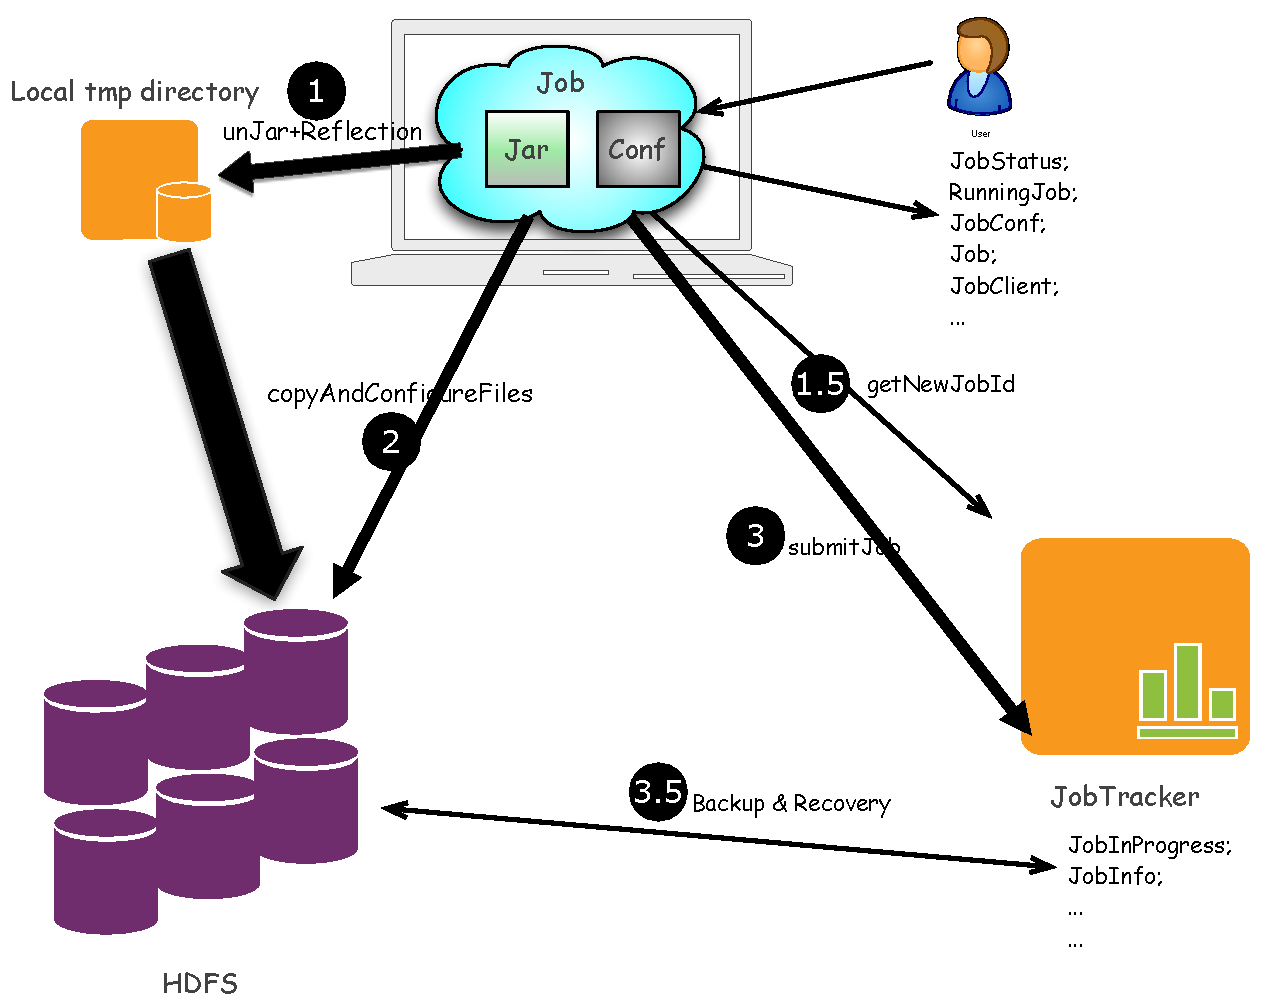
\includegraphics[height=4.2in, width=4.2in]{graphics/HadoopJobSubmit.pdf}
\label{mrj}
%\caption{MR Job Submit Procedure}
\end{figure}

Above Figure shows the major steps in submitting a MapReduce job in a
jar file:
\begin{enumerate}
\item RunJar class will unjar the jar file into local temporary
  directory
\item Call JobTracker's RPC interface to obtain a new jobId, and the
  remote directory
\item copy these jar file and associate files into HDFS
\item call JobTracker's RPC interface 'submitJob' to do the real work
\item backup current jobinfo in JobTracker to do recovery in future
\end{enumerate}

\bibliography{sample-handout}
\bibliographystyle{plainnat}


\printindex

\end{document}

